\subsubsection{Общая информация}

FPGA состоит из:
\begin{itemize}
  \item Логических блоков, реализующих базовые операции
  \item Блоков ввода-вывода
  \item Внутренних связей
\end{itemize}

Логические блоки имеют некоторое количество входов и выходов, реализуя
произвольную логическую функцию от соответствующего числа аргументов на любом
своем выходе.

Блоки ввода-вывода обеспечивают связь между контактами корпуса и внутренними
связями.

Внутренние связи организованы в виде вертикальных и горизонтальных каналов,
состоящих из нескольких связей. На пересечении каналов находятся блоки
переключения, позволяющие подключать связи из канала, входящего в блок к
соответствующим связям из оставшихся трех каналов. Схема блока переключения,
находящегося на пересечении четырех связей, показана на рисунке \ref{fpga-cell}.

\begin{figure}
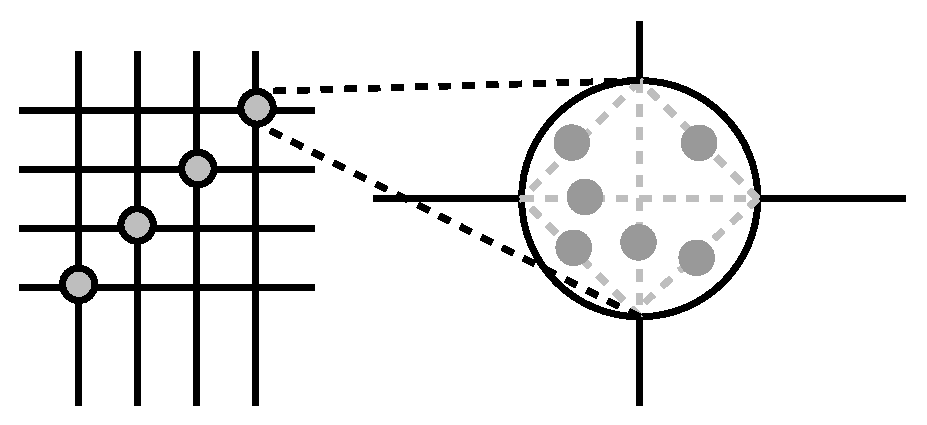
\includegraphics [width=\textwidth]{pictures/cell}
\caption{Схема блока переключения FPGA}
\label{fpga-cell}
\end{figure}

\subsubsection{Задачи, решаемые на FPGA}

В данное время, основные производители FPGA устройств такие как Xilinx и Altera
предлагают свои решения для различных областей рынка, таких как:

\begin{enumerate}
	\item Аэрокосмическая
	\item Оборонная
	\item Автомобильная
	\item Сфера обслуживания
	\item Высокопроизводительные вычисления
	\item Хранение данных
	\item Проводные и беспроводные соединения
	\item Автоматизация индустриальных процессов
	\item Медицинская
	\item Телекоммуникационная
\end{enumerate}

Фактически, все эти решения предполагаю использования FPGA в одном из следующих
вариантов:

\begin{enumerate}
  \item Независимое вычислительное устройство(stand - alone)
  		\begin{enumerate}
  		  \item Цифровая обработка сигналов(DSP)
  		  		Долгое время FPGA не могли сравниться в производительности с DSP
  		  		процессорами, но постепенное развитие: увеличение числа логических
  		  		блоков, появления специализированных DSP блоков, добавление
  		  		мультиплексоров, повышение тактовой частоты, позволили стать
  		  		конкурентноспособными. Кроме того, на определённых задачах, возможности
  		  		параллельной обработки, дают резкий прирост производительности.

  		  \item Реализация логики управления некоторым устройством.
  		  		Электронные устройства или некоторая система из них нуждается в
  		  		непосредственном управлении. Разумеется, можно использовать для этого
  		  		ASIC устройства, однако цена такого решения высока. Потому огромной
  		  		популярностью пользуются реализации на FPGA устройствах. 
  		  		Наиболее широко используются такие решения в силовая
  		  		электронике. К примеру, в самолёте Airbus 380 находится
  		  		по меньшей мере 700 FPGA чипов. Согласно проведённым исследованиям,
  				добавление логики управления на FPGA чипе для всех электромоторов в США,
  				позволит экономить в год 15 млрд. \$.
  		\end{enumerate}
  \item Акселератор
  		Аппаратная реализация алгоритма, широкие возможности для параллельного
  		исполнения, экономное энергопотребление делают устройство привлекательным
  		для выполнения как научных так и прикладных вычислений. Существуют уже
  		готовые вычислительные системы состоящие как из обычных центральных
  		процессоров так и блоков FPGA акселераторов Примерами прикладных задач
  		являются: декодирование видео и аудио потоков, криптографические задачи,
  		ускорение работы баз данных, обработка финансовых данных.
  \item Прототипирование
    	FPGA являются основой текущей мейнстримовой методологии аппаратной
  		верификации ASIC и SoC а также раннего проектирования проектирования
  		программного обеспечения и прошивок. Компания Intel проектировала на системе
  		FPGA кристаллов процессоры Intel Atom и Intel Nehalem. 
\end{enumerate}

